\section{Рабочий проект}
\subsection{Классы, используемые при разработке сайта}

Список классов и методов, которые были использованы при создании приложения представлены на таблице \ref{class:table}.

\renewcommand{\arraystretch}{0.8} % уменьшение расстояний до сетки таблицы
\begin{xltabular}{\textwidth}{|X|p{2.5cm}|>{\setlength{\baselineskip}{0.7\baselineskip}}p{4.85cm}|>{\setlength{\baselineskip}{0.7\baselineskip}}p{4.85cm}|}
\caption{Описание классов, используемых в приложении\label{class:table}}\\
\hline \centrow \setlength{\baselineskip}{0.7\baselineskip} Название класса & \centrow \setlength{\baselineskip}{0.7\baselineskip} Модуль, к которому относится класс & \centrow Описание класса & \centrow Методы \\
\hline \centrow 1 & \centrow 2 & \centrow 3 & \centrow 4\\ \hline
\endfirsthead
\caption*{Продолжение таблицы \ref{class:table}}\\
\hline \centrow 1 & \centrow 2 & \centrow 3 & \centrow 4\\ \hline
\finishhead
ANFIS & Нейронная сеть & ANFIS – класс, в котором осуществляется идентификация объектов с использованием нечеткой нейросети. & нормализацияКаналов( ПутьФайла)

Происходит загрузка изображения из файла, последующее его разделение на цветовые каналы, а затем преобразование этих каналов, представленных в виде матриц, в массивы. После этого происходит нормализация значений яркости.

АнфисаРаспознать( Путь, ИмяМодели)

В рамках данной функции осуществляется прием данных, обработанных методом нормализацияКаналов.\\
\hline & & & Эти данные, совмещенные с оптимизированной моделью искусственной нейронной сети, подвергаются дальнейшей обработке в модуле anfisReady, который разработан на основе программного обеспечения MATLAB. Завершающим этапом является генерация черно-белой маски, которая визуализирует распознанные объекты и имеет разрешение 720x720 пикселей

АнфисаТренировать( Набор, Размер, ИмяМодели)

Инициируя процесс обучения, функция использует предоставленный набор данных и его объем для конфигурации модуля anfis, реализованного в среде MATLAB. На основании этих данных функция строит и оптимизирует модель нечеткой нейронной сети. После успешного обучения, сформированная модель сохраняется в базу данных с наименованием, указанным в параметрах функции.\\
\hline & & & function out = AnfisReady(data, name)
 
Данная функция, реализованная на языке программирования MATLAB и использующая среду выполнения MATLAB Runtime, осуществляет передачу данных в нейронную сеть на пиксельном уровне. В соответствии с выбранной моделью нейросети, функция вычисляет степень соответствия каждого пикселя заданной модели и возвращает количественную оценку этого соответствия.

function out = Anfis(data, name)

Программный модуль, реализованный на языке программирования MATLAB и эксплуатирующий среду выполнения MATLAB Runtime, предназначен для приема набора данных, представляющих собой тренировочную выборку. Данный модуль осуществляет процесс обучения нечеткой нейронной сети, используя предоставленные данные.\\
\hline & & & В результате выполнения, модуль выдает модель нечеткой нейронной сети, прошедшую процедуру обучения.\\
\hline DB & База данных & DB – Класс для работы с базой данных & сохранить(ИмяМодели, Набор)

Данная функция реализует процедуру архивации тренировочного датасета и соответствующей обученной нейросетевой модели в структурированное хранилище данных. Это обеспечивает сохранность исходных обучающих данных и параметров модели для последующего использования и анализа.

загрузитьСписокНаборов()

Функциональный модуль предназначен для извлечения данных из базы данных, содержащей информацию о тренировочных наборах и соответствующих обученных нейронных моделях.\\
\hline & & & Он выполняет операцию чтения и последующего формирования перечня доступных тренировочных наборов данных и ассоциированных с ними моделей.

загрузитьНабор(Название)

Эта функция осуществляет операцию извлечения из базы данных специфического обучающего набора, состоящего из трёх цветовых каналов и целевого значения.\\
\hline main & Графический интерфейс & main – Класс для взаимодействия с пользователем & загрузитьИзображение()

Данная функция выполняет загрузку изображения из файла, а затем проводит его масштабирование до определённых размеров 720x720 пикселей, что обеспечивает его корректное отображение в заданном графическом интерфейсе пользователя.\\
\hline & & & 

распознать()

Функция инициирует процесс передачи ранее загруженного изображения в архитектуру нейронной сети, после чего активирует интерфейс для выбора предварительно обученной модели из доступных вариантов, что позволяет пользователю взаимодействовать с системой машинного обучения.

выбрать(ОкноВыбора)

Данная функция осуществляет интеграцию предварительно обученной модели в структуру нейронной сети, после чего производит деактивацию интерфейса выбора.

сохранитьРезультатРаспознания()

Функция инициирует активацию диалогового интерфейса, предназначенного для сохранения выходных данных нейронной сети в файловую систему, обеспечивая тем самым персистентность результатов вычислений.\\
\hline & & & 

обучать()

Функция активирует пользовательский интерфейс в виде диалогового окна, которое предоставляет возможность выбора набора данных для обучения нейронной сети.

подтвердить(ОкноВыбора)

Функция инициирует передачу выбранного или вновь созданного датасета для обучения нейронной сети, после чего активируется интерфейс в виде диалогового окна, предоставляющего пользователю опцию присвоения наименования новой модели.

отправить(ОкноНазвания)

Эта функция осуществляет трансмиссию наименования модели в архитектуру нейронной сети, инициируя этим процедуру обучения.\\
\hline & & & По завершении процесса, модель систематически регистрируется и архивируется в соответствующей базе данных, что обеспечивает её доступность для дальнейшего использования и интеграции в различные прикладные задачи машинного обучения.
\end{xltabular}
\renewcommand{\arraystretch}{1.0} % восстановление сетки

\subsection{Модульное тестирование разработанного приложения}

Модульные тесты для класса ANFIS из модели данных представлены на рисунках \ref{test1:image}-\ref{test3:image}.

\begin{figure}[ht]
\begin{lstlisting}[language=Python]
import os
import unittest
from PIL import Image
import anfis
import numpy as np
import matlab
from random import shuffle
from ANFIS import нормализацияКаналов
from ANFIS import АнфисаРаспознать

class TestНормализацияКаналов(unittest.TestCase):
    def test_нормализация_существующего_файла(self):
        результат = нормализацияКаналов('test_image.png')
        self.assertIsNotNone(результат, "Функция должна возвращать не None для существующего файла")
        self.assertTrue((результат >= 0).all() and (результат <= 1).all(), "Все значения должны быть в диапазоне от 0 до 1")
    def test_нормализация_несуществующего_файла(self):
        результат = нормализацияКаналов('несуществующий_файл.jpg')
        self.assertIsNone(результат, "Функция должна возвращать None для несуществующего файла")
\end{lstlisting}  
\caption{Модульный тест метода нормализацияКаналов класса ANFIS}
\label{test1:image}
\end{figure}

\begin{figure}[ht]
\begin{lstlisting}[language=Python]
import os
import unittest
from PIL import Image
import anfis
import numpy as np
import matlab
from random import shuffle
from ANFIS import нормализацияКаналов
from ANFIS import АнфисаРаспознать

class TestАнфисаРаспознать(unittest.TestCase):
    def setUp(self):
        self.путь = 'test_image.png'
        self.имяМодели = 'test_model_name'
    def test_распознавание_изображения(self):
        результат = АнфисаРаспознать(self.путь, self.имяМодели)
        self.assertIsInstance(результат, Image.Image, "Функция должна возвращать объект изображения")
    def test_сохранение_изображения(self):
        результат = АнфисаРаспознать(self.путь, self.имяМодели)
        self.assertTrue(os.path.isfile('output_image.png'), "Файл изображения должен быть сохранён")
\end{lstlisting}  
\caption{Модульный тест метода АнфисаРаспознать класса ANFIS}
\label{test2:image}
\end{figure}

\begin{figure}[ht]
\begin{lstlisting}[language=Python]
import os
import unittest
from PIL import Image
import anfis
import numpy as np
import matlab
from random import shuffle
from ANFIS import нормализацияКаналов
from ANFIS import АнфисаРаспознать

class TestНормализацияКаналов(unittest.TestCase):
    def test_нормализация_существующего_файла(self):
        результат = нормализацияКаналов('test_image.png')
        self.assertIsNotNone(результат, "Функция должна возвращать не None для существующего файла")
        self.assertTrue((результат >= 0).all() and (результат <= 1).all(), "Все значения должны быть в диапазоне от 0 до 1")
    def test_нормализация_несуществующего_файла(self):
        результат = нормализацияКаналов('несуществующий_файл.jpg')
        self.assertIsNone(результат, "Функция должна возвращать None для несуществующего файла")
\end{lstlisting}  
\caption{Модульный тест метода нормализацияКаналов класса ANFIS}
\label{test3:image}
\end{figure}

Модульные тесты для класса DB из модели данных представлены на рисунках \ref{test4:image}-\ref{test6:image}.

\begin{figure}[ht]
\begin{lstlisting}[language=Python]
from DB import сохранить
from DB import загрузитьСписокНаборов
from DB import загрузитьНабор

class TestСохранить(unittest.TestCase):
    def setUp(self):
        self.ИмяМодели = 'test_model'
        self.Набор = [(1, 2, 3, 4), (5, 6, 7, 8)]
        self.Подключение = sqlite3.connect(':memory:')
        self.Курсор = self.Подключение.cursor()
        self.Курсор.execute('''CREATE TABLE Готовые_данные (Адрес_файла TEXT)''')
        self.Курсор.execute('''CREATE TABLE Тренировочный_набор (Красный_канал INTEGER, Синий_канал INTEGER, Зелёный_канал INTEGER, Выходные_данные INTEGER)''')
        self.Курсор.execute('''CREATE TABLE Модель (Имя_модели TEXT, ИД_Тренировочного_набора INTEGER, ИД_Готовых_данных INTEGER)''')
    def test_подключение_к_базе(self):
        self.assertIsNotNone(self.Подключение, "Должно быть установлено подключение к базе данных")
    def test_добавление_в_готовые_данные(self):
        сохранить(self.ИмяМодели, self.Набор)
        self.Курсор.execute("SELECT * FROM Готовые_данные WHERE Адрес_файла = ?", (self.ИмяМодели,))
        результат = self.Курсор.fetchone()
        self.assertIsNotNone(результат, "Модель должна быть добавлена в таблицу Готовые_данные")
    def test_добавление_в_тренировочный_набор(self):
        сохранить(self.ИмяМодели, self.Набор)
        for данные in self.Набор:
            self.Курсор.execute("SELECT * FROM Тренировочный_набор WHERE Красный_канал = ? AND Синий_канал = ? AND Зелёный_канал = ? AND Выходные_данные= ?", данные)
            результат = self.Курсор.fetchone()
            self.assertIsNotNone(результат, "Данные должны быть добавлены в таблицу Тренировочный_набор")
    def test_закрытие_подключения(self):
        self.Подключение.close()
        self.assertRaises(sqlite3.ProgrammingError, self.Курсор.execute, "SELECT * FROM Готовые_данные")
    def tearDown(self):
        self.Подключение.close()
\end{lstlisting}  
\caption{Модульный тест метода загрузитьНабор класса DB}
\label{test4:image}
\end{figure}

\begin{figure}[H]
\begin{lstlisting}[language=Python]
from DB import сохранить
from DB import загрузитьСписокНаборов
from DB import загрузитьНабор

class TestЗагрузитьСписокНаборов(unittest.TestCase):
    def setUp(self):
        self.Подключение = sqlite3.connect(':memory:')
        self.Курсор = self.Подключение.cursor()
        self.Курсор.execute('''CREATE TABLE Готовые_данные (Адрес_файла TEXT)''')
        self.Курсор.executemany("INSERT INTO Готовые_данные (Адрес_файла) VALUES (?)", [('file1',), ('file2',), ('file3',)])

    def test_загрузка_списка(self):
        ожидаемый_список = ['file1', 'file2', 'file3']
        результат = загрузитьСписокНаборов()
        self.assertEqual(результат, ожидаемый_список, "Список наборов должен соответствовать ожидаемому")

    def test_закрытие_подключения(self):
        загрузитьСписокНаборов()
        self.assertRaises(sqlite3.ProgrammingError, self.Курсор.execute, "SELECT * FROM Готовые_данные")

    def tearDown(self):
        self.Подключение.close()
\end{lstlisting}  
\caption{Модульный тест метода загрузитьСписокНаборов класса DB}
\label{test5:image}
\end{figure}

\begin{figure}[H]
\begin{lstlisting}[language=Python]
from DB import сохранить
from DB import загрузитьСписокНаборов
from DB import загрузитьНабор

class TestЗагрузитьНабор(unittest.TestCase):
    def setUp(self):
        Название = 'test_model'
        self.Подключение = sqlite3.connect(':memory:')
        self.Курсор = self.Подключение.cursor()
        self.Курсор.execute('''CREATE TABLE Модель (Имя_модели TEXT, ИД_Тренировочного_набора INTEGER)''')
        self.Курсор.execute('''CREATE TABLE Тренировочный_набор (ИД_тренировочного_набора INTEGER, Красный_канал INTEGER, Синий_канал INTEGER, Зелёный_канал INTEGER, Выходные_данные INTEGER)''')
        self.Курсор.execute("INSERT INTO Модель (Имя_модели, ИД_Тренировочного_набора) VALUES (?, ?)", (Название, 1))
        self.Курсор.execute("INSERT INTO Тренировочный_набор (ИД_тренировочного_набора, Красный_канал, Синий_канал, Зелёный_канал, Выходные_данные) VALUES (1, 255, 0, 0, 1)")

    def test_загрузка_набора(self):
        ожидаемый_выход = [(255, 0, 0, 1)]
        результат = загрузитьНабор('test_model')
        self.assertEqual(результат[0], ожидаемый_выход, "Загруженный набор должен соответствовать ожидаемому")

    def test_формат_выходных_данных(self):
        результат = загрузитьНабор('test_model')
        self.assertEqual(результат[1], (1, 4), "Формат выходных данных должен быть кортежем с размерностью набора")

    def test_закрытие_подключения(self):
        загрузитьНабор('test_model')
        self.assertRaises(sqlite3.ProgrammingError, self.Курсор.execute, "SELECT * FROM Модель")

    def tearDown(self):
        self.Подключение.close()
\end{lstlisting}  
\caption{Модульный тест метода загрузитьНабор класса DB}
\label{test6:image}
\end{figure}
\subsection{Системное тестирование разработанного приложения}

На рисунке \ref{systemtest_interface:image} представлен интерфейс программы.
\begin{figure}[H]
\centering
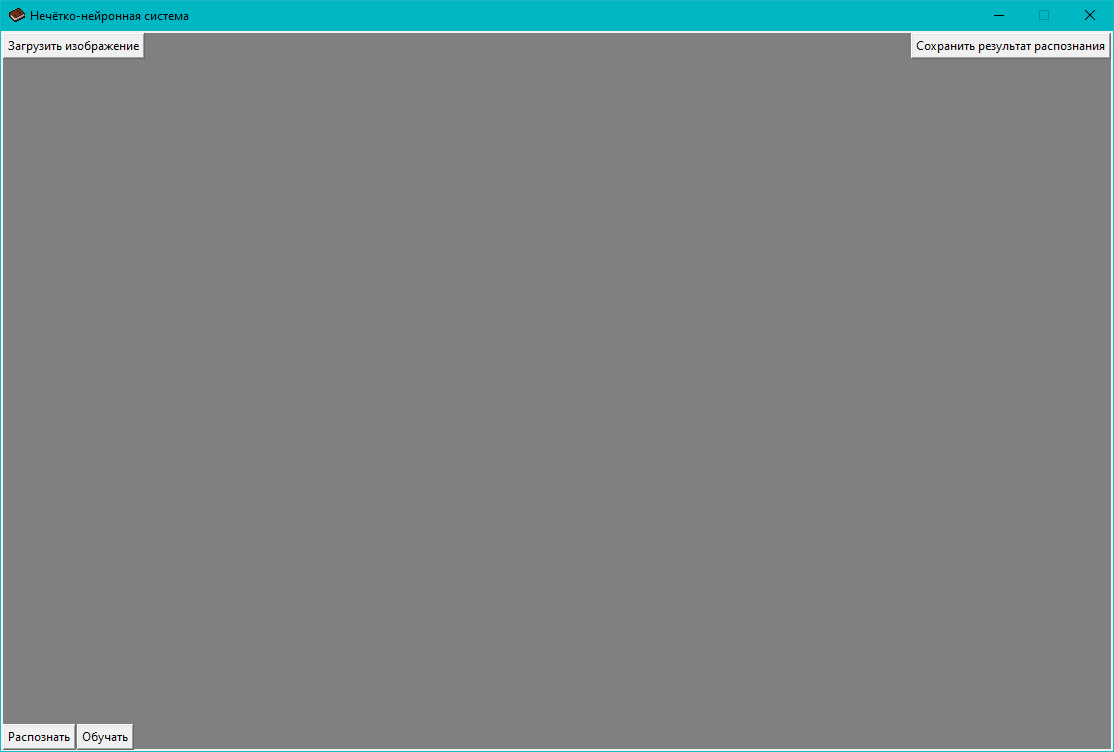
\includegraphics[width=1\linewidth]{systemtest_interface}
\caption{Диаграмма вариантов использования}
\label{systemtest_interface:image}
\end{figure}

На рисунках \ref{systemtest_responce:image}-\ref{systemtest_responce4:image} представлен полный путь распознания объекта на изображении.

\begin{figure}[H]
\center{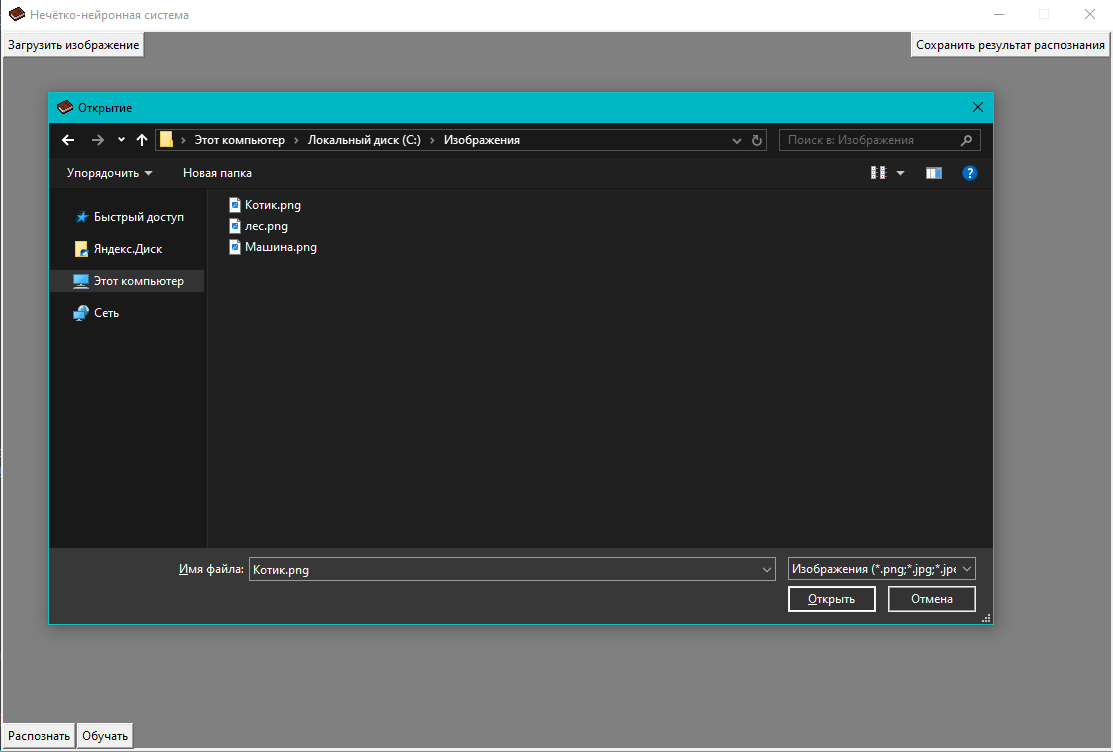
\includegraphics[width=1\linewidth]{systemtest_responce}}
\caption{Диалоговое окно загрузки файла Машина.png}
\label{systemtest_responce:image}
\end{figure}

\begin{figure}[H]
\center{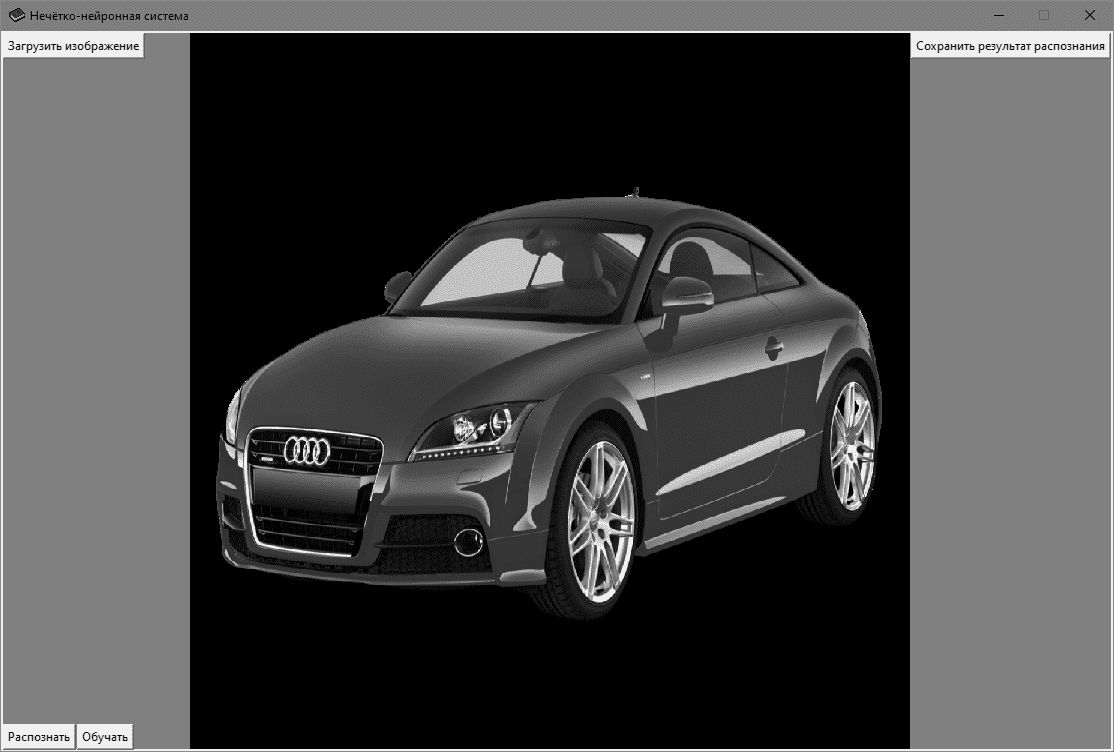
\includegraphics[width=1\linewidth]{systemtest_responce1}}
\caption{Изображение отображено в интерфейсе программы}
\label{systemtest_responce1:image}
\end{figure}

\begin{figure}[H]
\center{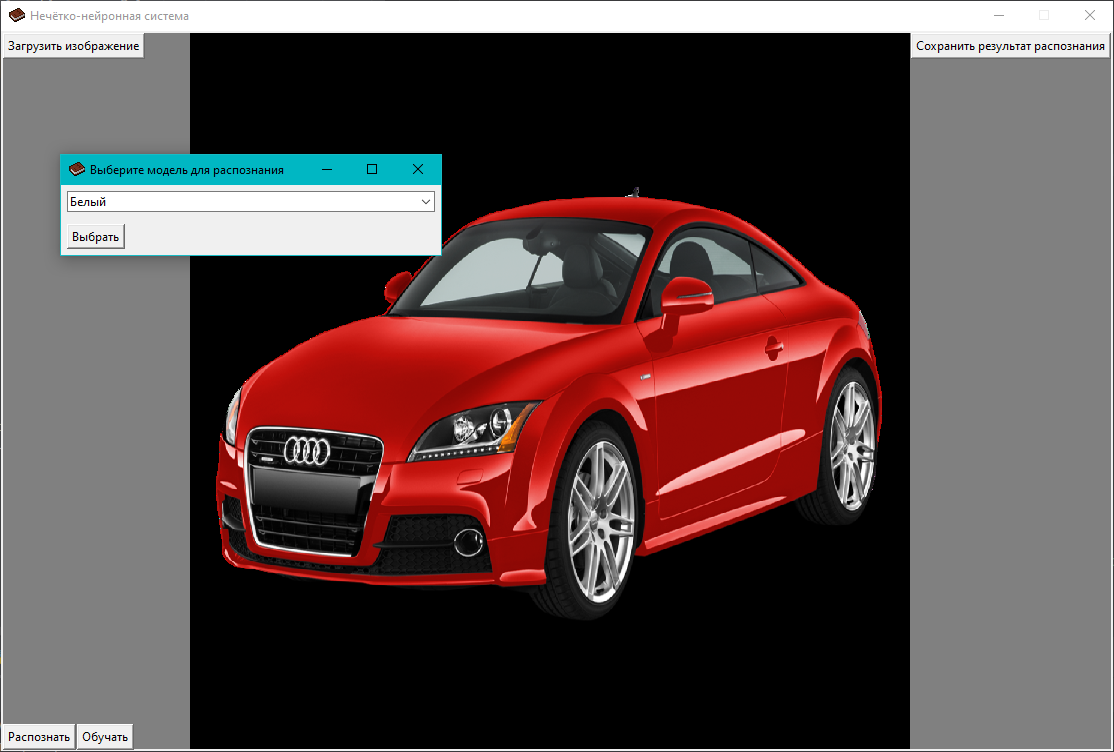
\includegraphics[width=1\linewidth]{systemtest_responce2}}
\caption{Окно выбора модели для распознания}
\label{systemtest_responce2:image}
\end{figure}

\begin{figure}[H]
\center{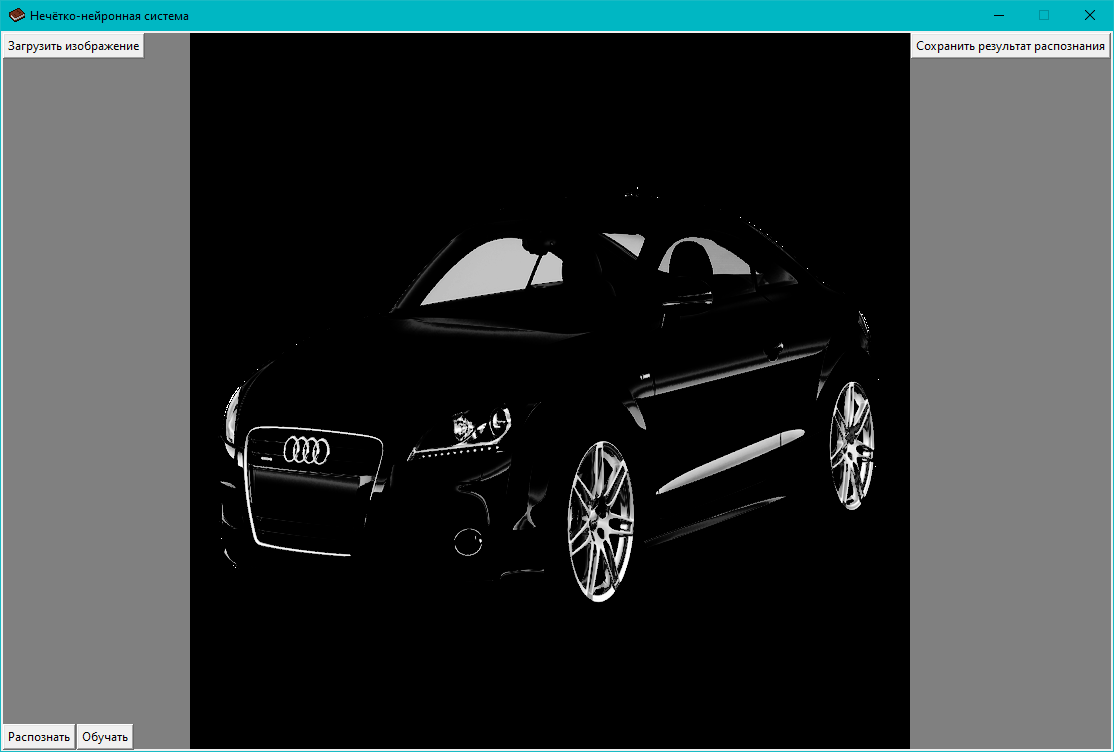
\includegraphics[width=1\linewidth]{systemtest_responce3}}
\caption{Распознанный объект отображен на интерфейсе}
\label{systemtest_responce3:image}
\end{figure}

\begin{figure}[H]
\center{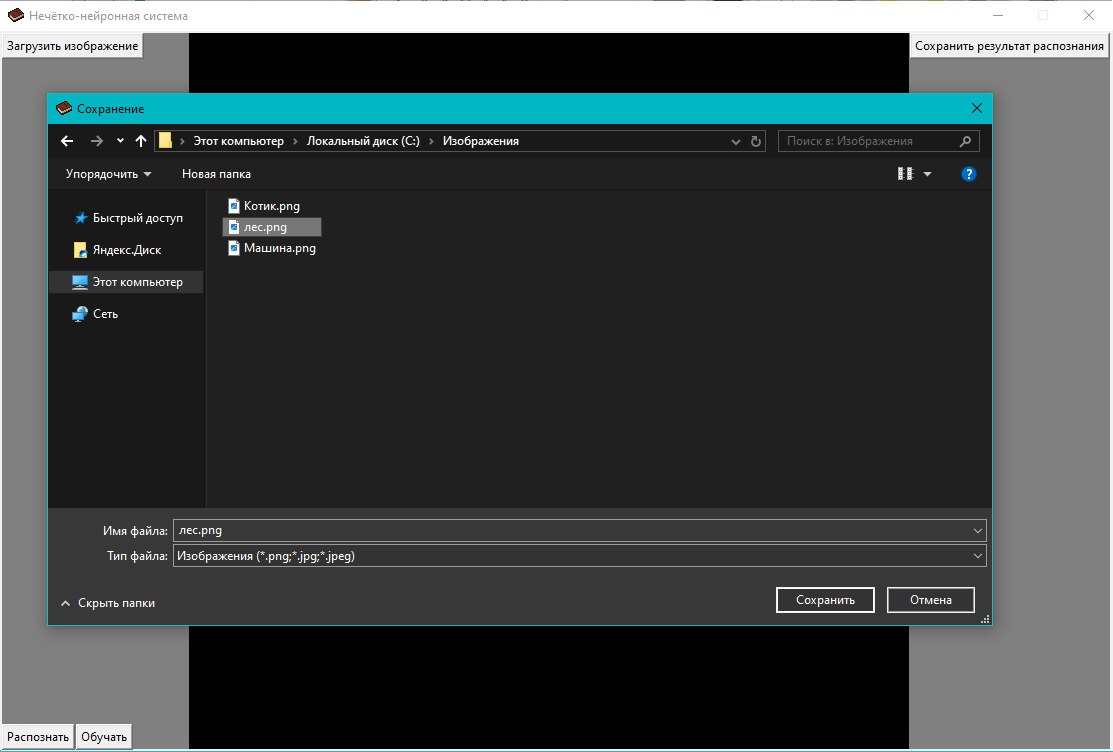
\includegraphics[width=1\linewidth]{systemtest_responce4}}
\caption{Диалоговое окно сохранения результата}
\label{systemtest_responce4:image}
\end{figure}

На рисунках \ref{systemtest_train1:image}-\ref{systemtest_train3:image} представлены все варианты обучения нейронной сети.

На рисунке \ref{systemtest_train1:image} была нажата кнопка обучать, после чего открылось окно выбора набора.

\begin{figure}[H]
\center{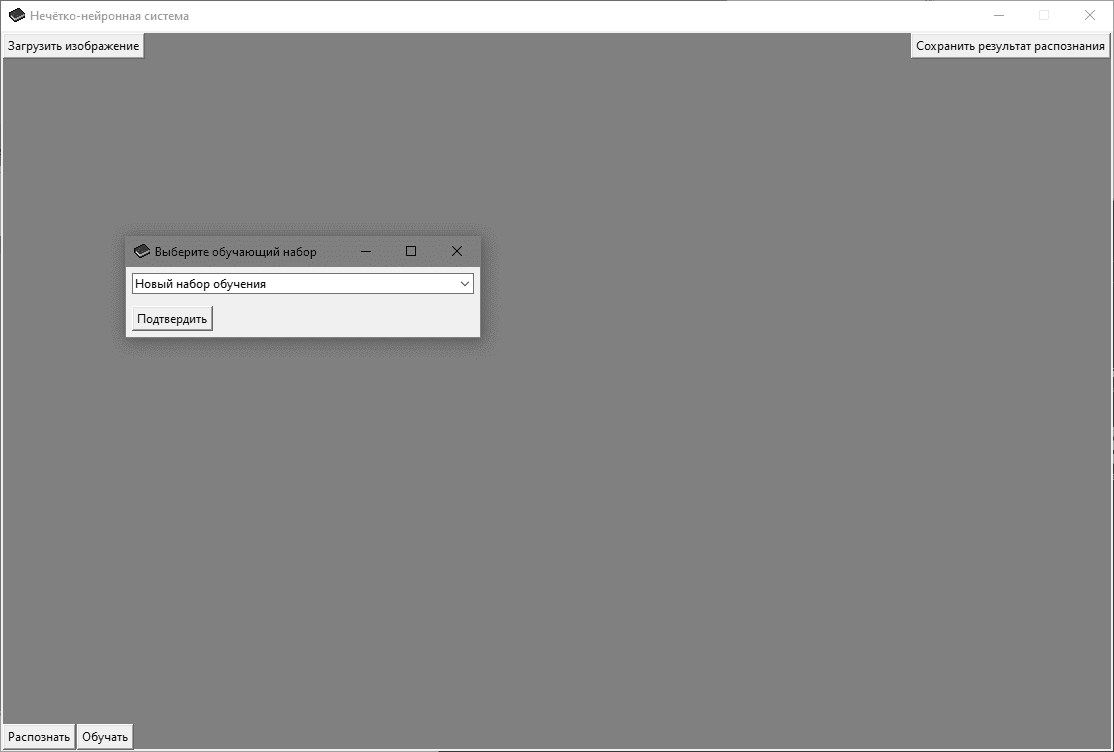
\includegraphics[width=1\linewidth]{systemtest_train1}}
\caption{Окно выбора обучающего набора}
\label{systemtest_train1:image}
\end{figure}

После выбора нового набора появилось окно, предлагающее назвать модель и обучить её.

\begin{figure}[H]
\center{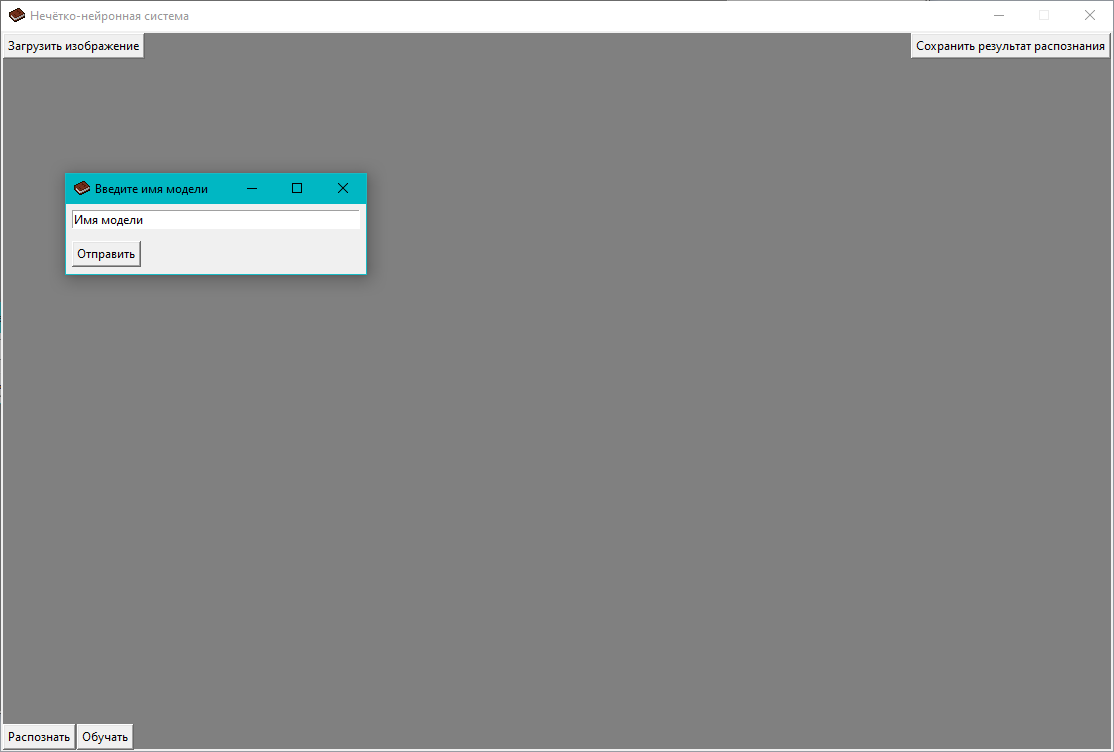
\includegraphics[width=1\linewidth]{systemtest_train2}}
\caption{Окно выбора названия новой модели}
\label{systemtest_train2:image}
\end{figure}

Вместо создания нового набора, после нажатия кнопки обучать, можно выбрать заготовленный набор и обучить нейронную сеть по нему.

\begin{figure}[H]
\center{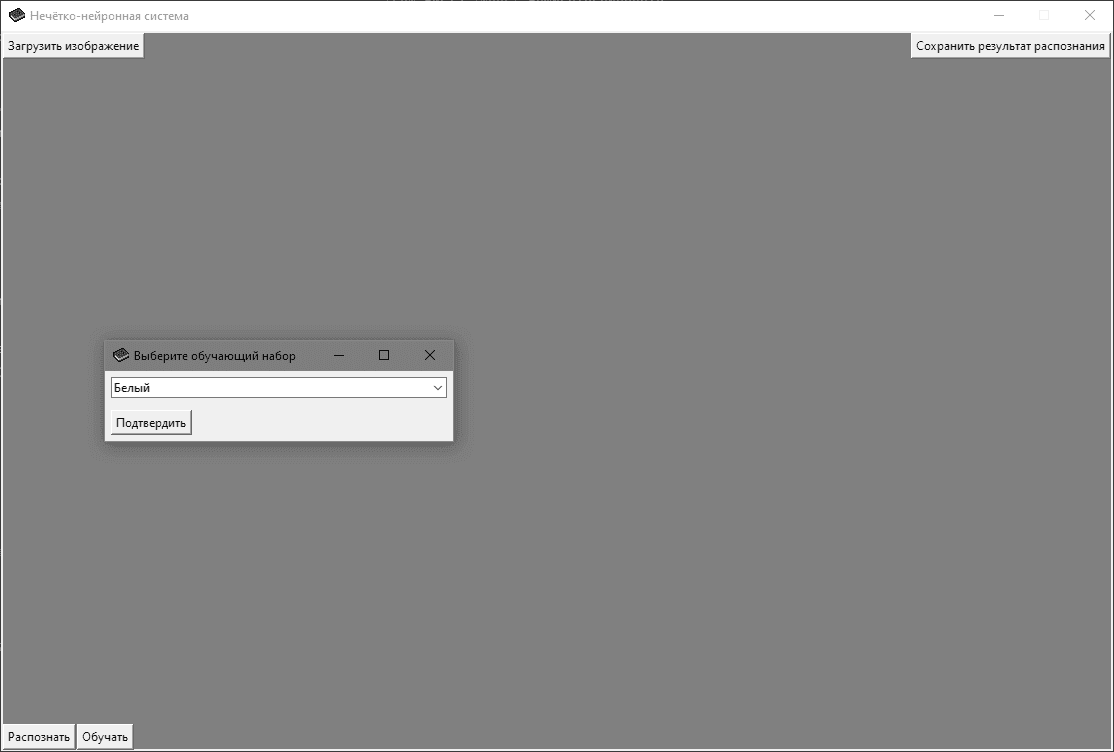
\includegraphics[width=1\linewidth]{systemtest_train3}}
\caption{Выбор обучения по набору ''Белый''}
\label{systemtest_train3:image}
\end{figure}

На рисунке \ref{systemtest_responce5:image} было загружено изображение кошки.

\begin{figure}[H]
\center{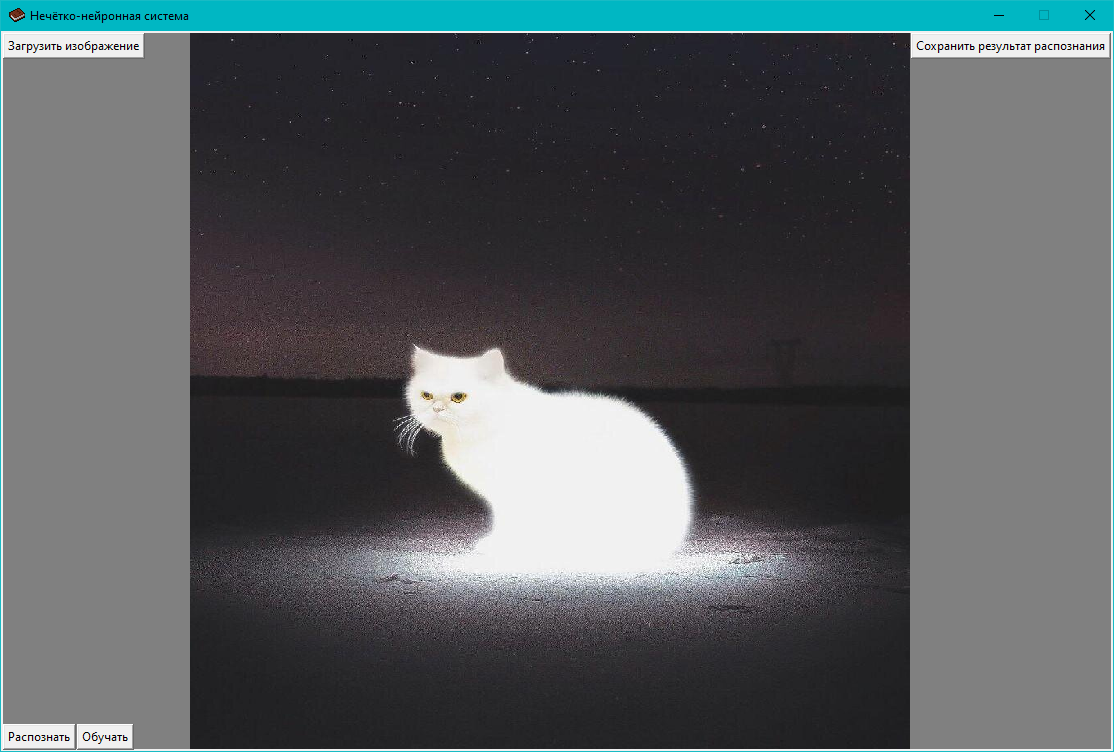
\includegraphics[width=1\linewidth]{systemtest_responce5}}
\caption{Интерфейс с изображением кошки}
\label{systemtest_responce5:image}
\end{figure}

На рисунке \ref{systemtest_responce6:image} изображение кошки было обработано по модели ''Белый''.

\begin{figure}[H]
\center{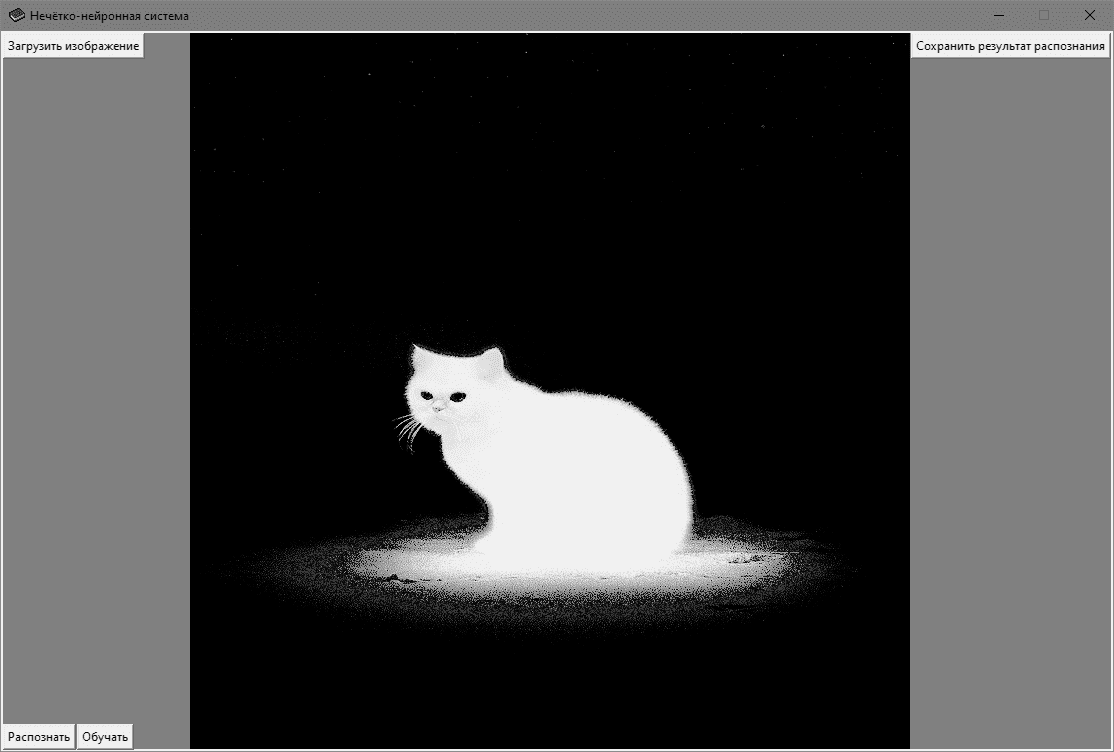
\includegraphics[width=1\linewidth]{systemtest_responce6}}
\caption{Распознанныйе объекты на изображении кошки}
\label{systemtest_responce6:image}
\end{figure}
На рисунке \ref{systemtest_responce7:image} было загружено изображение лилии.

\begin{figure}[H]
\center{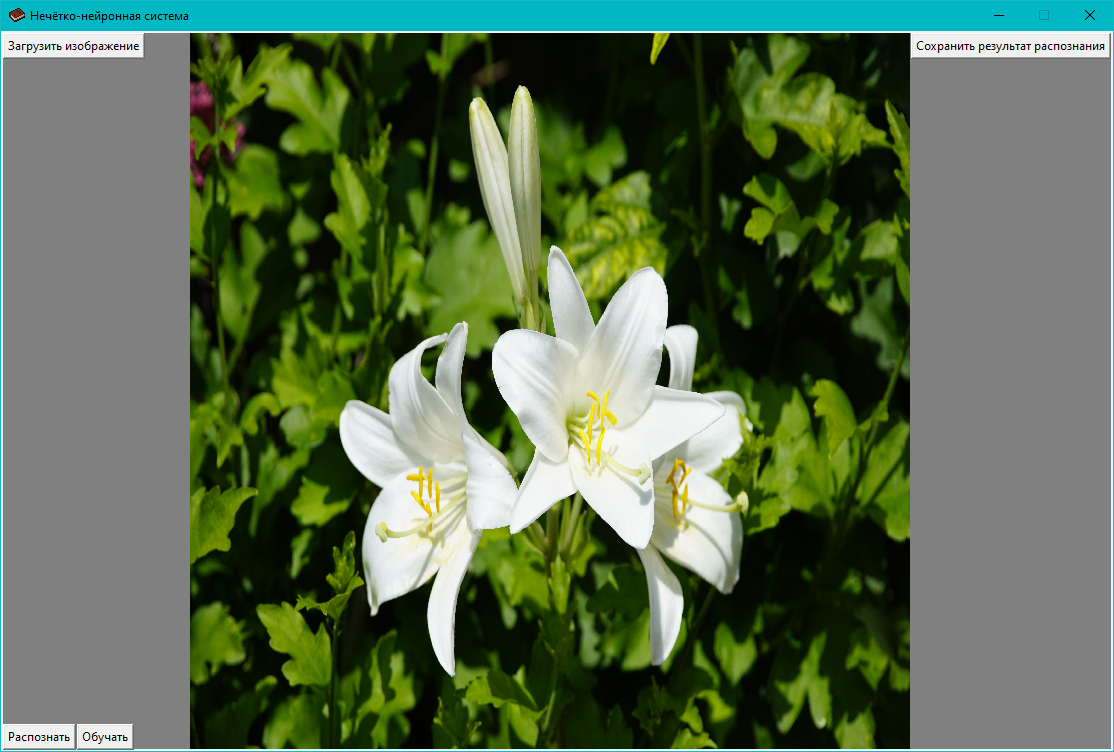
\includegraphics[width=1\linewidth]{systemtest_responce7}}
\caption{Интерфейс с изображением лилии}
\label{systemtest_responce7:image}
\end{figure}

На рисунке \ref{systemtest_responce8:image} изображение лилии было обработано по модели ''Белый''.

\begin{figure}[H]
\center{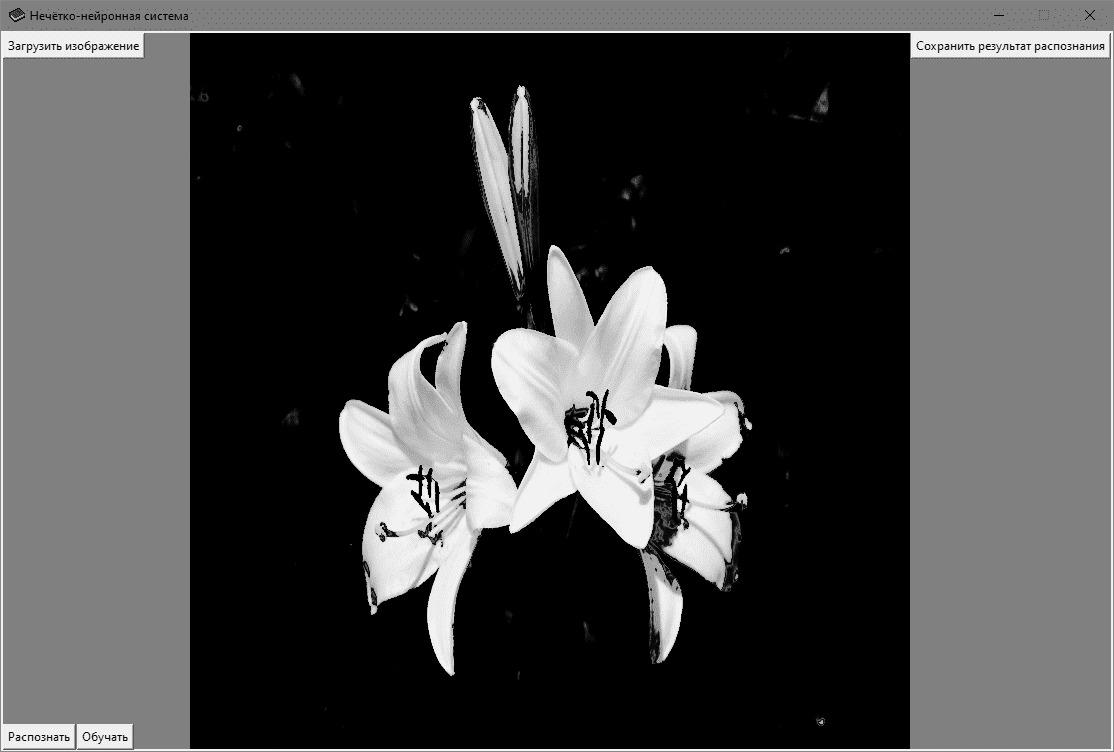
\includegraphics[width=1\linewidth]{systemtest_responce8}}
\caption{Распознанныйе объекты на изображении лилии}
\label{systemtest_responce8:image}
\end{figure}
На рисунке \ref{systemtest_responce9:image} было загружено изображение леса.

\begin{figure}[H]
\center{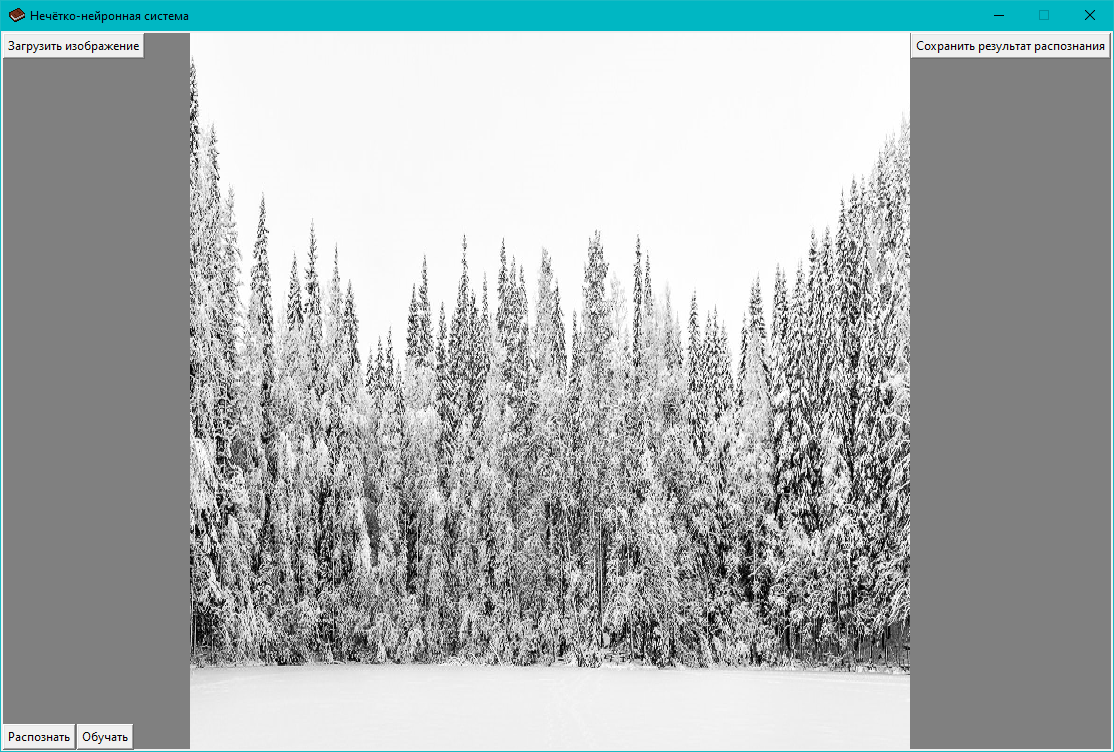
\includegraphics[width=1\linewidth]{systemtest_responce9}}
\caption{Интерфейс с изображением леса}
\label{systemtest_responce9:image}
\end{figure}

На рисунке \ref{systemtest_responce10:image} изображение леса было обработано по модели ''Белый''.

\begin{figure}[H]
\center{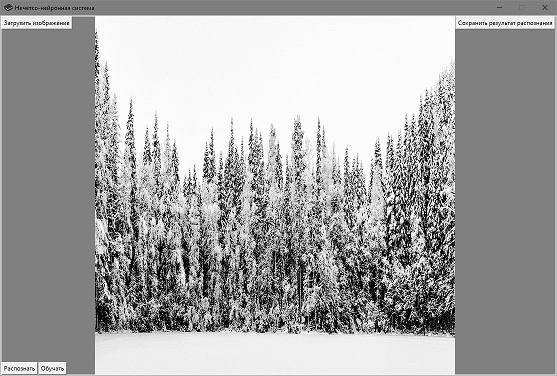
\includegraphics[width=1\linewidth]{systemtest_responce10}}
\caption{Распознанныйе объекты на изображении леса}
\label{systemtest_responce10:image}
\end{figure}
На рисунке \ref{systemtest_responce11:image} было загружено изображение футбола.

\begin{figure}[H]
\center{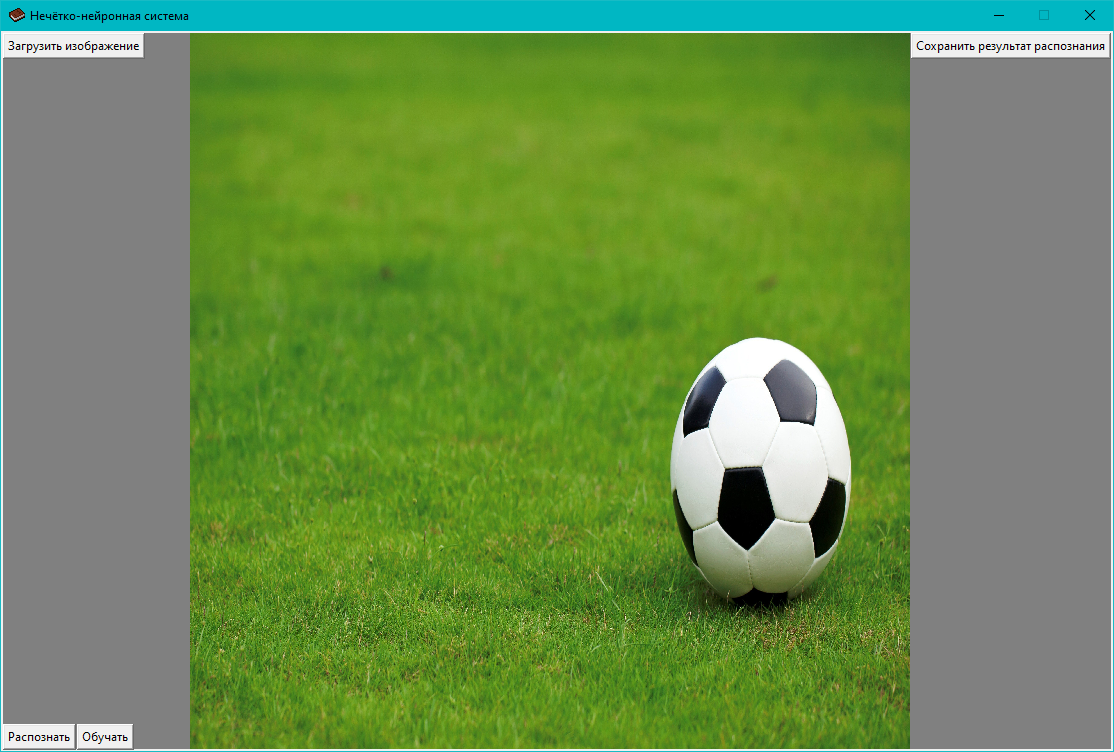
\includegraphics[width=1\linewidth]{systemtest_responce11}}
\caption{Интерфейс с изображением футбола}
\label{systemtest_responce11:image}
\end{figure}

На рисунке \ref{systemtest_responce12:image} изображение футбола было обработано по модели ''Белый''.

\begin{figure}[H]
\center{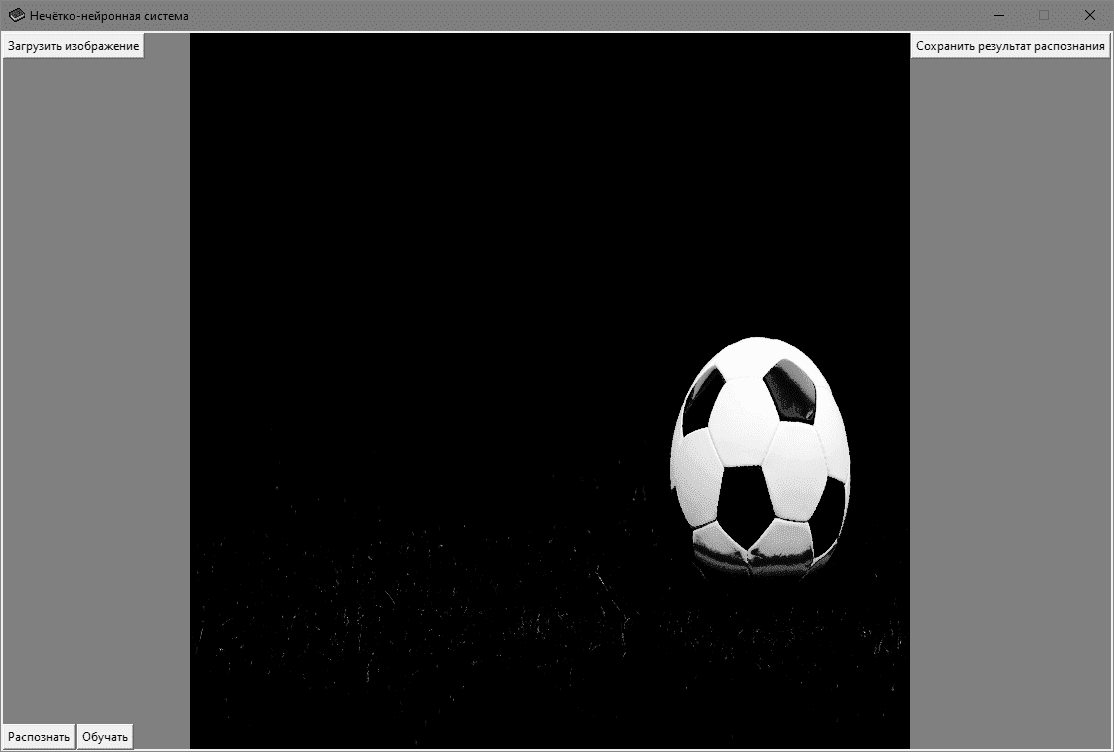
\includegraphics[width=1\linewidth]{systemtest_responce12}}
\caption{Распознанныйе объекты на изображении футбола}
\label{systemtest_responce12:image}
\end{figure}
На рисунке \ref{systemtest_responce13:image} было загружено изображение платья.

\begin{figure}[H]
\center{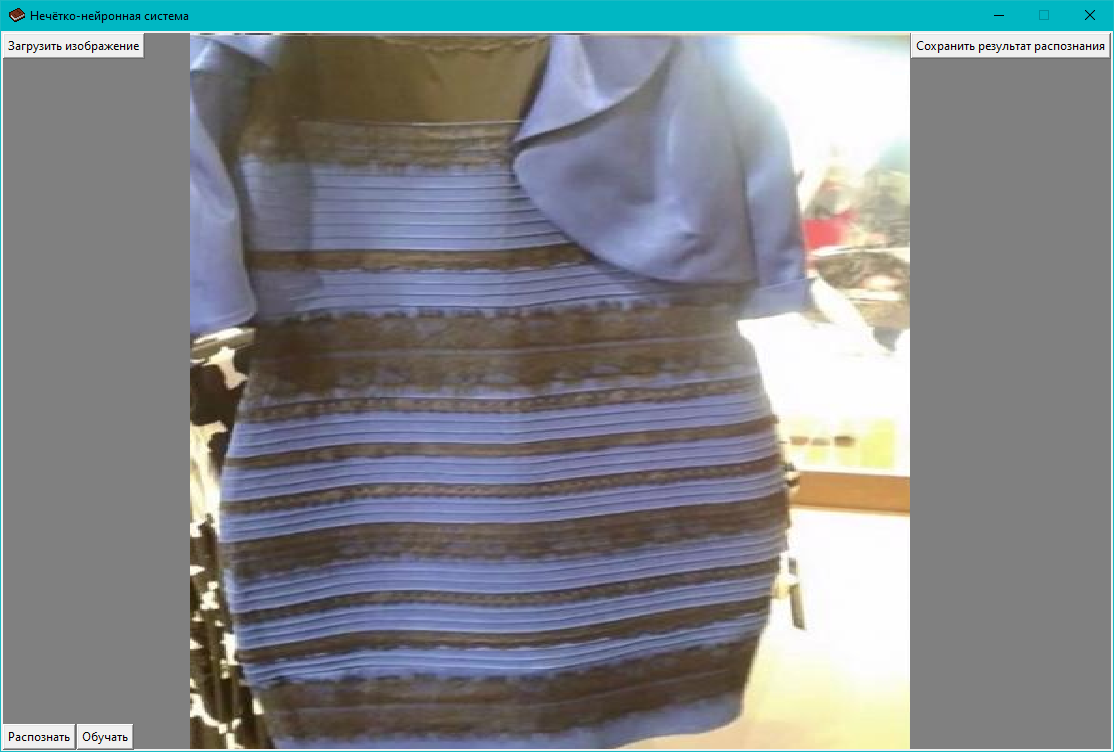
\includegraphics[width=1\linewidth]{systemtest_responce13}}
\caption{Интерфейс с изображением платья}
\label{systemtest_responce13:image}
\end{figure}

На рисунке \ref{systemtest_responce14:image} изображение платья было обработано по модели ''Белый''.

\begin{figure}[H]
\center{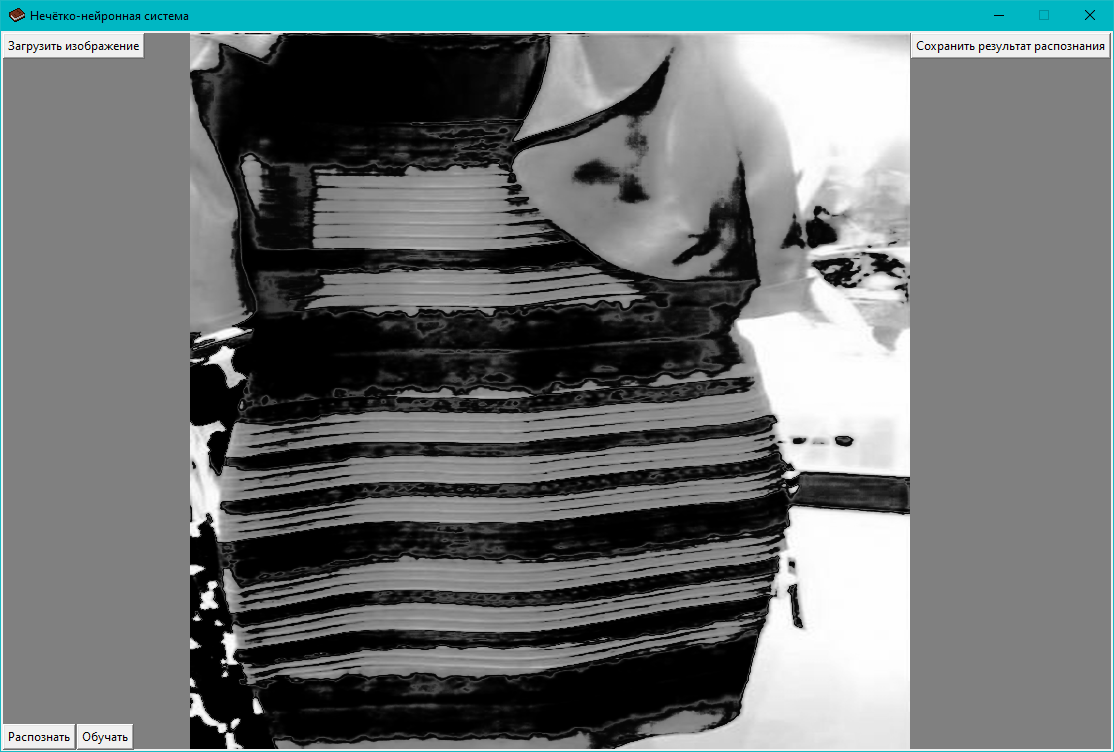
\includegraphics[width=1\linewidth]{systemtest_responce14}}
\caption{Распознанныйе объекты на изображении платья}
\label{systemtest_responce14:image}
\end{figure}

На рисунке \ref{systemtest_responce15:image} было загружено изображение берёзы.

\begin{figure}[H]
\center{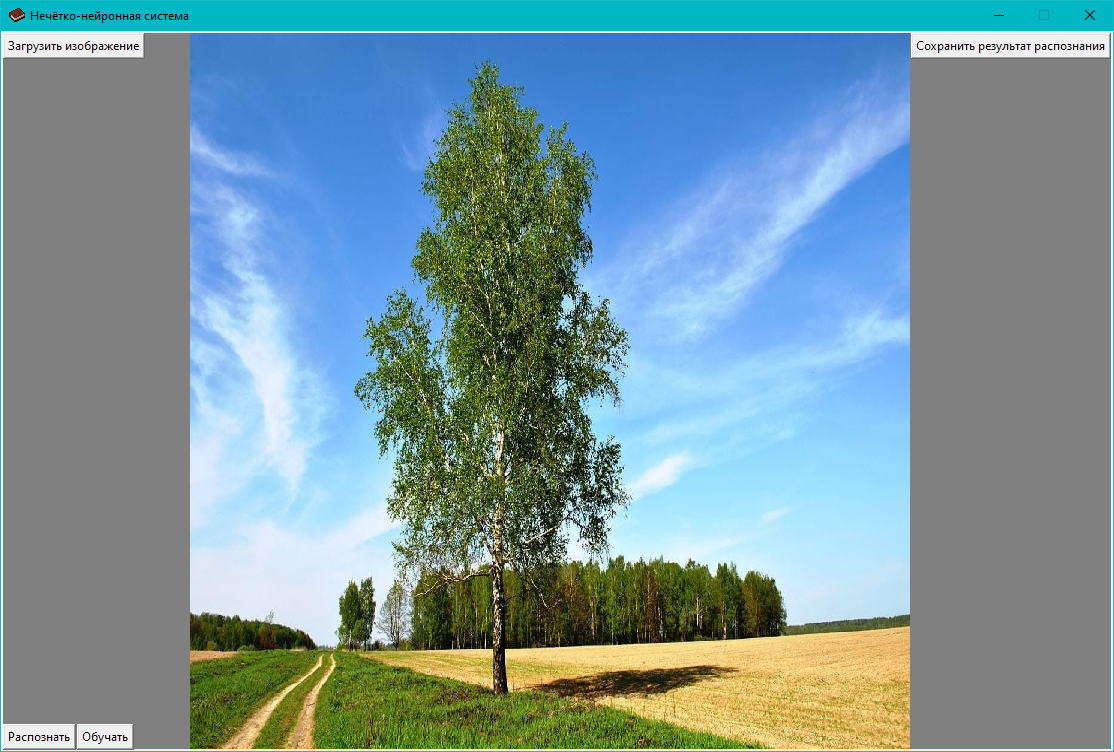
\includegraphics[width=1\linewidth]{systemtest_responce15}}
\caption{Интерфейс с изображением берёзы}
\label{systemtest_responce15:image}
\end{figure}

На рисунке \ref{systemtest_responce16:image} изображение берёзы было обработано по модели ''Белый''.

\begin{figure}[H]
\center{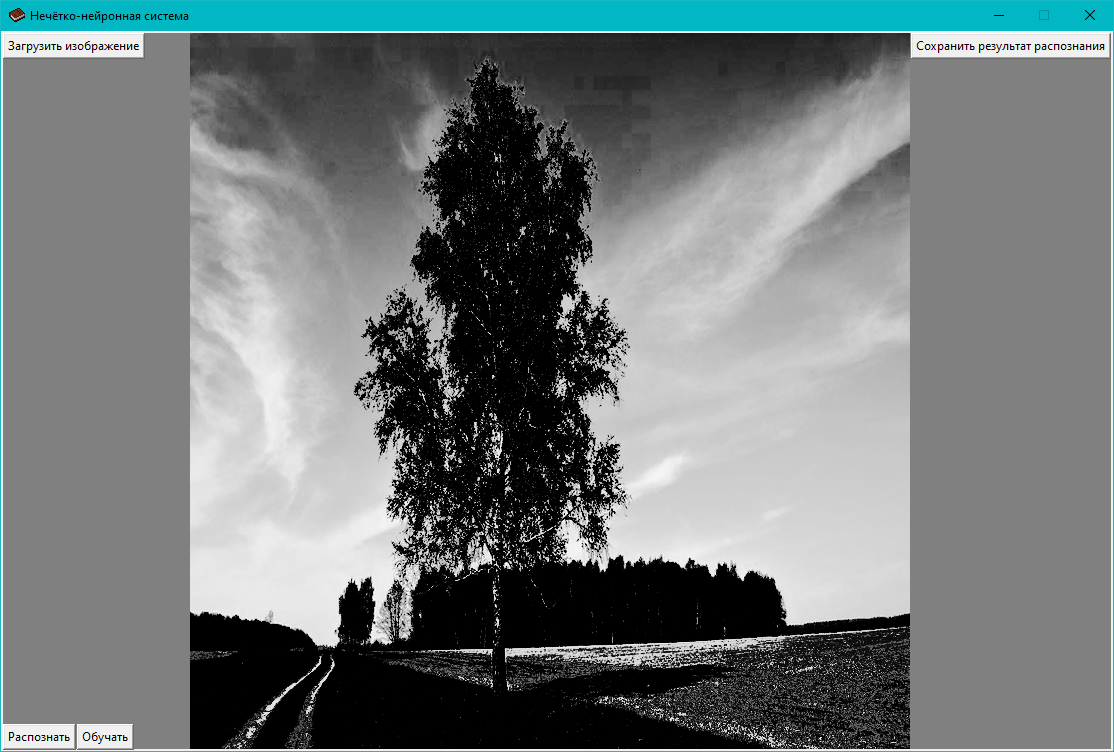
\includegraphics[width=1\linewidth]{systemtest_responce16}}
\caption{Распознанныйе объекты на изображении берёзы}
\label{systemtest_responce16:image}
\end{figure}